
\section{The \pkg{sbtools} package}

With \pkg{sbtools}, our goal was to allow complete
access to the ScienceBase web service API in a flexible, lightweight
R package. The package imports a minimal number of external packages
to support core functionality. More advanced data access (e.g., geospatial
web services) is supported through suggested packages to keep the basic
installation requirements minimal for all platforms. Within R, \pkg{sbtools}
is designed to keep end-user interactions simple despite the underlying 
complexity of many of the web service calls (e.g., authentication).

Below, we describe briefly the core functions available in \pkg{sbtools}
and discuss the unique features of ScienceBase that \pkg{sbtools}
exposes to R users.


\subsection{Data access API}
The data access functionality of \pkg{sbtools} makes it easy to
access any public item. Every item in ScienceBase has a unique identifier
that can be used for direct access to the item and its associated data and
metadata. A lightweight representation of this information is created in R
with the \code{item\_get} function.

\noindent\rule{\textwidth}{0.4pt}
\begin{example}
> test_item = item_get("4f4e4b24e4b07f02db6aea14")
> test_item
<ScienceBase Item>
  Title: Coastal-change and glaciological maps of Antarctica
  Creator/LastUpdatedBy:      /
  Provenance (Created / Updated):  2010-10-06T04:25:43Z / 2014-07-21T17:45:42Z
  Children: FALSE
  Item ID: 4f4e4b24e4b07f02db6aea14
  Parent ID: 4f4e4771e4b07f02db47e1e4
\end{example}
\noindent\rule{\textwidth}{0.4pt}

This representation is defined by \pkg{sbtools} as an \code{sbitem} object,
which contains many fields and can be further inspected in the same
way as a named list.

\noindent\rule{\textwidth}{0.4pt}
\begin{example}
> names(test_item)
 [1] "link"              "relatedItems"      "id"
 [4] "identifiers"       "title"             "citation"
 [7] "provenance"        "hasChildren"       "parentId"
[10] "contacts"          "webLinks"          "browseCategories"
[13] "browseTypes"       "tags"              "dates"
[16] "facets"            "files"             "distributionLinks"
[19] "previewImage"

> test_item$citation
[1] "Geological Survey (U.S.), 1999-08-05, Coastal-change
and glaciological maps of Antarctica:  Fact SheetCoastal-change and
glaciological maps of Antarctica."
\end{example}
\noindent\rule{\textwidth}{0.4pt}

On ScienceBase, the hierarchical item tree dictates relationships between items; 
each item has one parent and potentially many children. \pkg{sbtools} allows the user to
easily traverse this tree structure. Because ScienceBase allows users to define their internal 
organization, this heirarchy can take on different meanings for different projects, including 
conveying data provenance or spatial grouping.

% we could consider adding functions to get the actual parent and child
% items rather than just their IDs - e.g., item_get_parent() returns one sbitem
% and item_get_children() returns a list of sbitems. Save the user from wrapping
% all this in item_get() calls.

\noindent\rule{\textwidth}{0.4pt}
\begin{example}
#parent ID always available as item attribute
> parent = item_get(test_item$parentId)
> parent
  Title: USGS Publications Warehouse
  Creator/LastUpdatedBy:      /
  Provenance (Created / Updated):  2012-02-29T15:42:41Z / 2014-07-08T21:42:20Z
  Children: TRUE
  Item ID: 4f4e4771e4b07f02db47e1e4
  Parent ID: 4f4e4771e4b07f02db47e1da

#getting sibling items
> item_list_children(parent)
[1] "55b98fbee4b08f6647be5179" "541d45a4e4b0f68901ec30ef"
[3] "55b361b3e4b09a3b01b5daad" "53516ef9e4b05569d8059f34"
[5] "4f4e4ab2e4b07f02db66f5e3" "5351704ee4b05569d805a2e4"
\end{example}
\noindent\rule{\textwidth}{0.4pt}

ScienceBase items may have data or metadata files attached to them.
You can list and download attached files directly using \pkg{sbtools}.

\noindent\rule{\textwidth}{0.4pt}
\begin{example}
#returns names of files attached to item
> item_list_files(test_item)
                              fname size  url
  1 metadata6644450227216673613.xml 1742  https://www.sciencebase.gov/[truncated]

#returns local path to downloaded files
> item_file_download(test_item, dest_dir = tempdir())
[1] "\\path\\to\\file\\RtmpgBV2fn/metadata6644450227216673613.xml"
\end{example}
\noindent\rule{\textwidth}{0.4pt}

ScienceBase has special functionality for certain data types.
One example is spatial data. When spatial data uploaded to ScienceBase 
and appropriate metadata is included, they can be accessed using 
Open Geospatial Consortium (\href{http://www.opengeospatial.org/}{OGC}) 
web services. \pkg{sbtools} has includes functionality to access Web
Feature Service (WFS) when available. Note: Some formatting details of code
omitted from code below for simplicity. See demo('', package='') for full
example.

\noindent\rule{\textwidth}{0.4pt}
\begin{example}
#Load non-sbtools-required but useful mapping packages
library(maps)
library(sp)
#an item with an included OGC WFS service
layer = item_get_wfs('55e372b9e4b05561fa208212')
map('state', regions = 'iowa')
plot(layer, add = TRUE)
\end{example}
\noindent\rule{\textwidth}{0.4pt}

%this figure code is demo\figure_map_code.R
% feel free to improve
 \begin{figure}[htbp]
   \centering
   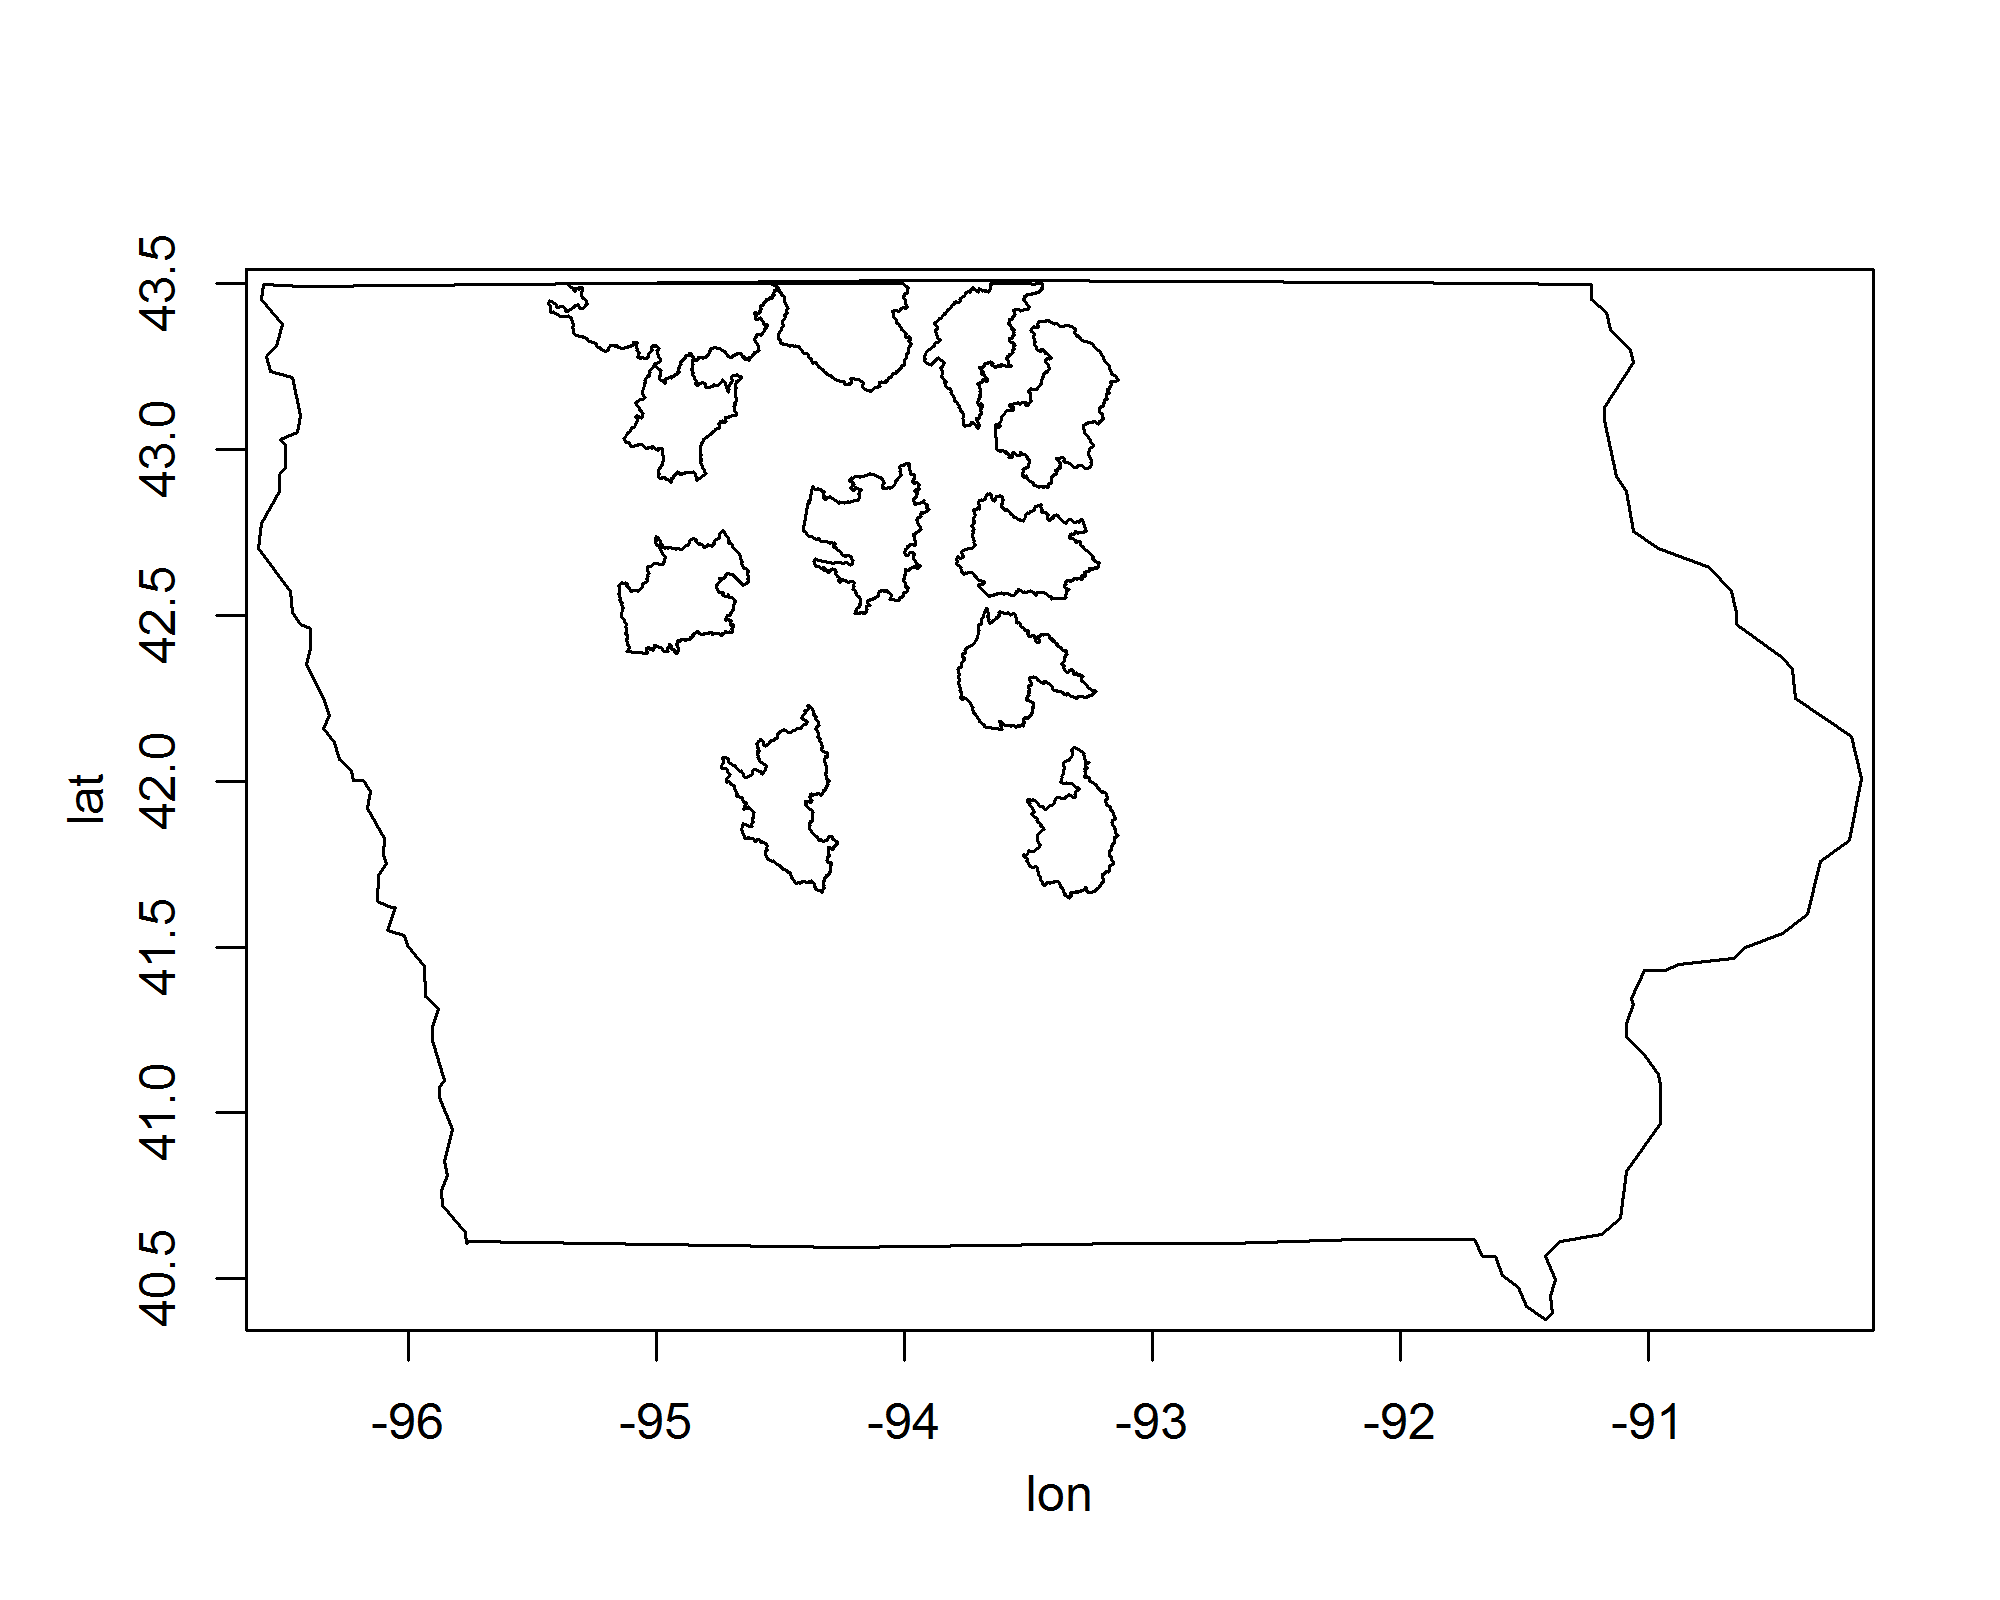
\includegraphics{mapfig}
   \caption{An example spatial dataset from ScienceBase. 
   Shows high priority regions in Iowa containing shallow
   lakes and marshes to create management emphasis areas 
   for migratory water fowl habitat.}
   \label{figure:iowafig}
 \end{figure}


\subsection{Search API}
To support advanced and powerful data discovery, all datasets
in ScienceBase are indexed and made available through a flexible
search interface. \pkg{sbtools} offers several query
functions with different levels of search specificity, from
cross-metadata simple text search to low-level, metadata specific search
functionality.

In \pkg{sbtools}, query functions are included to support the most common query types. 
Included functions are available to search based on free-text, project folder, 
date-time range, geospatial
bounding box, Digital Object Identifier (DOI), and data type. To save space in
the examples below, we use the \code{limit} parameter to limit all queries to
the first one or two results. Further details for each query type are available in the
package documentation.


The ScienceBase free-text search is simple to use and generic as it 
searches across all of an item's text-based metadata fields. Free-text 
search can find specific text strings in almost all metadata fields, including 
but not limited to filenames, summary fields, citation, contacts, and authors. 
Spatial reference metadata is an example of a field not searched through the 
free-text search. Using \pkg{sbtools}, a free-text 
search can be run with the \code{query\_sb\_text} function.

\noindent\rule{\textwidth}{0.4pt}
\begin{example}
> query_sb_text('Antarctica', limit=1)
[[1]]
<ScienceBase Item> 
  Title: Antarctica. Erratic near camp 13. December 12, 1977.
  Creator/LastUpdatedBy:      / 
  Provenance (Created / Updated):  2013-07-09T15:38:45Z / 2016-03-02T23:55:43Z
  Children: FALSE
  Item ID: 51dc2e85e4b0f81004b79cf0
  Parent ID: 519ba0a3e4b0e4e151ef5dd9
\end{example}
\noindent\rule{\textwidth}{0.4pt}

Items can also be queried according to their position in the hierarchical item
tree. For example, projects funded by USGS Climate Science Centers each have sections on ScienceBase
where project information is stored. Using the web interface (and some user knowledge), we first found the
ScienceBase ID of the Northeast Climate Science Center community folder. Then, \pkg{sbtools} can be used 
to look for specific items in that commuinty. Below is an example of looking for 
items containing any reference to "Lake Superior" under the Northeast Climate Science Center community. 

\noindent\rule{\textwidth}{0.4pt}
\begin{example}
#Look for items referencing "Lake Superior" under the NE Climate Science Center projects
> query_item_in_folder("Lake Superior", folder="4f8c648de4b0546c0c397b43", limit=2)
[[1]]	
<ScienceBase Item> 
  Title: The Role of Lake-Dotted Landscapes in Regional Climate Change [...]
  Creator/LastUpdatedBy:      / 
  Provenance (Created / Updated):  2013-12-31T17:46:16Z / 2013-12-31T17:46:16Z
  Children: FALSE	
  Item ID: 52c302e8e4b040b25da9d35a
  Parent ID: 51db0ebce4b010c7f6a814bf

[[2]]
<ScienceBase Item> 
  Title: The influence of land use and [...] in Lake Superior tributaries
  Creator/LastUpdatedBy:      / 
  Provenance (Created / Updated):  2013-12-31T17:45:51Z / 2013-12-31T17:45:51Z
  Children: FALSE
  Item ID: 52c302cfe4b040b25da9ce3c
  Parent ID: 51db0ebce4b010c7f6a814bf
\end{example}
\noindent\rule{\textwidth}{0.4pt}

Date-time information for ScienceBase items may include the date of
data creation, modification, report, collection, and/or
publication. \pkg{sbtools} users may search any of these
date-time fields using the \code{date\_type} argument to the
\code{query\_sb\_date()} function.

\noindent\rule{\textwidth}{0.4pt}
\begin{example}
#Query recently updated items
> query_sb_date(Sys.time()-as.difftime(7, units="days"), Sys.time(),
+    date_type='lastUpdated', limit=2)
[[1]]
<ScienceBase Item>
  Title: US Topo
  Creator/LastUpdatedBy:      /
  Provenance (Created / Updated):  2012-03-05T22:46:14Z / 2016-02-01T12:11:58Z
  Children: TRUE
  Item ID: 4f554236e4b018de15819c85
  Parent ID: 4f552e93e4b018de15819c51

[[2]]
<ScienceBase Item>
  Title: USGS US Topo 7.5-minute map for Boyer, IA 2013
  Creator/LastUpdatedBy:      /
  Provenance (Created / Updated):  2014-05-01T08:13:22Z / 2016-02-01T10:21:18Z
  Children: FALSE
  Item ID: 53620222e4b0c409c627ec57
  Parent ID: 5061bc99e4b0ce47085a8d03

#Query for data published in the 1970's
> query_sb_date(as.POSIXct('1970-01-01'), as.POSIXct('1980-01-01'),
+   date_type = 'Publication', limit = 2)
[[1]]
<ScienceBase Item>
  Title: Common marsh plants of the United States and Canada
  Creator/LastUpdatedBy:      /
  Provenance (Created / Updated):  2010-10-22T22:24:18Z / 2014-07-05T04:55:27Z
  Children: FALSE
  Item ID: 4f4e4b24e4b07f02db6ae651
  Parent ID: 4f4e4771e4b07f02db47e1e4

[[2]]
<ScienceBase Item>
  Title: Structure and mineralization of Precambrian rocks in the Galena-
         Roubaix district, Black Hills, South Dakota
  Creator/LastUpdatedBy:      /
  Provenance (Created / Updated):  2010-10-23T00:28:32Z / 2014-07-21T20:14:53Z
  Children: FALSE
  Item ID: 4f4e4b14e4b07f02db6a47a6
  Parent ID: 4f4e4771e4b07f02db47e1e4
\end{example}
\noindent\rule{\textwidth}{0.4pt}

Each item can be described by a data type tag. Because this field is free-text,
it can take on a number of different values. The function \code{sb\_datatypes()}
returns the list of currently used data type tags on ScienceBase.
\code{query\_sb\_datatype} can be used to query for items described with a
specific data type.

\noindent\rule{\textwidth}{0.4pt}
\begin{example}
#List first 50 available data types
> sb_datatypes(limit = 50)
 [1] "Application"               "ArcGIS Map Package"       
 [3] "ArcGIS REST Map Service"   "ArcGIS Service Definition"
 [5] "ArcIMS Catalog"            "ArcIMS Metadata"          
 [7] "BASIS+ Project"            "BASIS+ Subtask"           
 [9] "BASIS+ Task"               "Book Citation"            
[11] "Citation"                  "Clearinghouse"            
[13] "Collection"                "Conference Citation"      
[15] "Digital Map - Beta"        "Document"                 
[17] "Downloadable"              "Electronic Book Citation" 
[19] "GeoProcessing Service"     "GeoTIFF"  


#Query for USGS Reports
> query_sb_datatype('Report', limit = 2)
[[1]]
<ScienceBase Item> 
  Title: Final Memo for Structured decision-making to facilitate multi-stakeholder coastal conservation and restoration under climate change uncertainties: case study on barrier islands of the northern Gulf of Mexico
  Creator/LastUpdatedBy:      / 
  Provenance (Created / Updated):   / 
  Children: 
  Item ID: 565e07b3e4b071e7ea5435d0
  Parent ID: 5224e64fe4b0e4746d62af85

[[2]]
<ScienceBase Item> 
  Title: Correlation & Climate Sensitivity of Human Health and Environmental Indicators in the Salish Sea - Final Report
  Creator/LastUpdatedBy:      / 
  Provenance (Created / Updated):   / 
  Children: 
  Item ID: 557a1504e4b0c350d7b9a7e5
  Parent ID: 527c2bdae4b0050d7e26b7c5
\end{example}
\noindent\rule{\textwidth}{0.4pt}

On ScienceBase, the preferred way of storing an item's DOI is using 
the identifier field, and specifying the type as DOI.
\code{query\_sb\_doi()} can query those fields specifically for
a DOI when properly described. Here are examples of querying items by DOI on ScienceBase:

\noindent\rule{\textwidth}{0.4pt}
\begin{example}
#Two example DOI-specific queries
query_sb_doi('10.5066/F7M043G7')
[[1]]
<ScienceBase Item>
  Title: 2013 Raw Ground Penetrating Radar Data on Alaska's Glaciers
  Creator/LastUpdatedBy:      /
  Provenance (Created / Updated):  2015-06-15T16:55:03Z / 2015-12-15T20:39:06Z
  Children: TRUE
  Item ID: 557f0367e4b023124e8ef621
  Parent ID: 5474ec49e4b04d7459a7eab2

query_sb_doi('10.5066/F7Z60M35')
[[1]]
<ScienceBase Item> 
  Title: Raw Ground Penetrating Radar Data, Eureka Glacier, Alaska; 2013
  Creator/LastUpdatedBy:      / 
  Provenance (Created / Updated):  2015-06-25T22:10:38Z / 2016-02-18T21:20:42Z
  Children: FALSE
  Item ID: 558c7c5ee4b0b6d21dd654ca
  Parent ID: 557f0367e4b023124e8ef621
\end{example}
\noindent\rule{\textwidth}{0.4pt}

Items with a geospatial component to their data or metadata can be queried using a
Lat/Lon bounding box with the function \code{query\_sb\_spatial()}. The
bounding box may be directly specified with coordinates or indirectly specified
by supplying another spatial object whose bounding box should be used. Because
spatial functionality requires packages beyond those imported by \pkg{sbtools} by default,
the \pkg{sp} and \pkg{gdalUtils} packages must be installed to use these functions.

\noindent\rule{\textwidth}{0.4pt}
\begin{example}
##specify the lat/long corners of the bounding box
> query_sb_spatial(bb_min = c(-104.4, 37.5), bb_max = c(-95.1, 41.0), limit = 2)
[[1]]
<ScienceBase Item>
  Title: National Fish Habitat Partnership Data System
  Creator/LastUpdatedBy:      /
  Provenance (Created / Updated):  2012-02-29T15:42:43Z / 2015-11-12T20:19:30Z
  Children: TRUE
  Item ID: 4f4e4773e4b07f02db47e241
  Parent ID: 4f4e4760e4b07f02db47df9c

[[2]]
<ScienceBase Item>
  Title: Geo Data Portal Catalog
  Creator/LastUpdatedBy:      /
  Provenance (Created / Updated):  2015-02-12T22:03:18Z / 2015-11-24T22:38:06Z
  Children: TRUE
  Item ID: 54dd2326e4b08de9379b2fb1
  Parent ID: 4f4e4760e4b07f02db47df9c

##You can also use the bounding box of an sp spatial data object
#grab an sp object from a pre-determined ScienceBase Item
> layer = item_get_wfs('55e372b9e4b05561fa208212')

#get items in that bounding box
> query_sb_spatial(layer, limit = 2)
[[1]]
<ScienceBase Item>
  Title: National Fish Habitat Partnership Data System
  Creator/LastUpdatedBy:      /
  Provenance (Created / Updated):  2012-02-29T15:42:43Z / 2015-11-12T20:19:30Z
  Children: TRUE
  Item ID: 4f4e4773e4b07f02db47e241
  Parent ID: 4f4e4760e4b07f02db47df9c

[[2]]
<ScienceBase Item>
  Title: USGS Denver Library Photographic Collection
  Creator/LastUpdatedBy:      /
  Provenance (Created / Updated):  2013-05-21T16:28:19Z / 2016-01-04T15:44:20Z
  Children: TRUE
  Item ID: 519ba0a3e4b0e4e151ef5dd9
  Parent ID: 4f4e4771e4b07f02db47e1da
\end{example}
\noindent\rule{\textwidth}{0.4pt}

Lastly, \pkg{sbtools} offers advanced access to all query capabilities through
the \code{query\_sb()} function. \code{query\_sb()} provides a convenient wrapper that 
allows the user to supply a list of query parameters (options described in the documentation),
submits that query to ScienceBase and parses the output
into a list of \code{sbitem} objects. When necessary, \code{query\_sb()} 
also does proper result paging when the requested
return length (limit) is over 1000 items. All advanced search options can be experimented
with via the \href{https://www.sciencebase.gov/catalog/items/queryForm}
{online advanced search interface}.

\noindent\rule{\textwidth}{0.4pt}
\begin{example}

# query_sb can be used for combined search criteria
> query_sb(list(q = "water", folderId = '504216b9e4b04b508bfd337d', browserCategory = 'Image'), limit=2)
[[1]]
<ScienceBase Item>
  Title: Encyclopedia of Water Science
  Creator/LastUpdatedBy:      /
  Provenance (Created / Updated):  2013-04-18T15:06:38Z / 2013-04-18T15:06:38Z
  Children: FALSE
  Item ID: 51700bfee4b05024ef3cd4ef
  Parent ID: 504216b9e4b04b508bfd337d

[[2]]
<ScienceBase Item>
  Title: Introduction to special section on Impacts of Land Use Change on Water Resources
  Creator/LastUpdatedBy:      /
  Provenance (Created / Updated):  2013-04-18T15:07:35Z / 2013-04-18T15:07:35Z
  Children: FALSE
  Item ID: 51700c37e4b05024ef3cd4fd
  Parent ID: 504216b9e4b04b508bfd337d
\end{example}
\noindent\rule{\textwidth}{0.4pt}

Combining both the query functionality and direct spatial data access through WFS web services, 
below is an example of exploring multiple available datasets on ScienceBase. In this example, 
we query for lakes with the word "faults" in their description which also expose data 
through an OGC WFS web service. 

\noindent\rule{\textwidth}{0.4pt}
\begin{example}
#Source non-sbtools-required but useful mapping packages
library(sp)
library(maps)

faults = query_sb(list(q = "faults", browseType = "OGC WFS Layer"), limit = 20)

map('usa')
for(i in 1:length(faults)){
    layer = item_get_wfs(faults[[i]]$id)
    layer = spTransform(layer, CRS('+proj=longlat +datum=WGS84'))
    plot(layer, add=TRUE, col='red')
}
map.axes()

\end{example}
\noindent\rule{\textwidth}{0.4pt}

%this figure code is demo\figure_fault_code.R
 \begin{figure}[htbp]
   \centering
   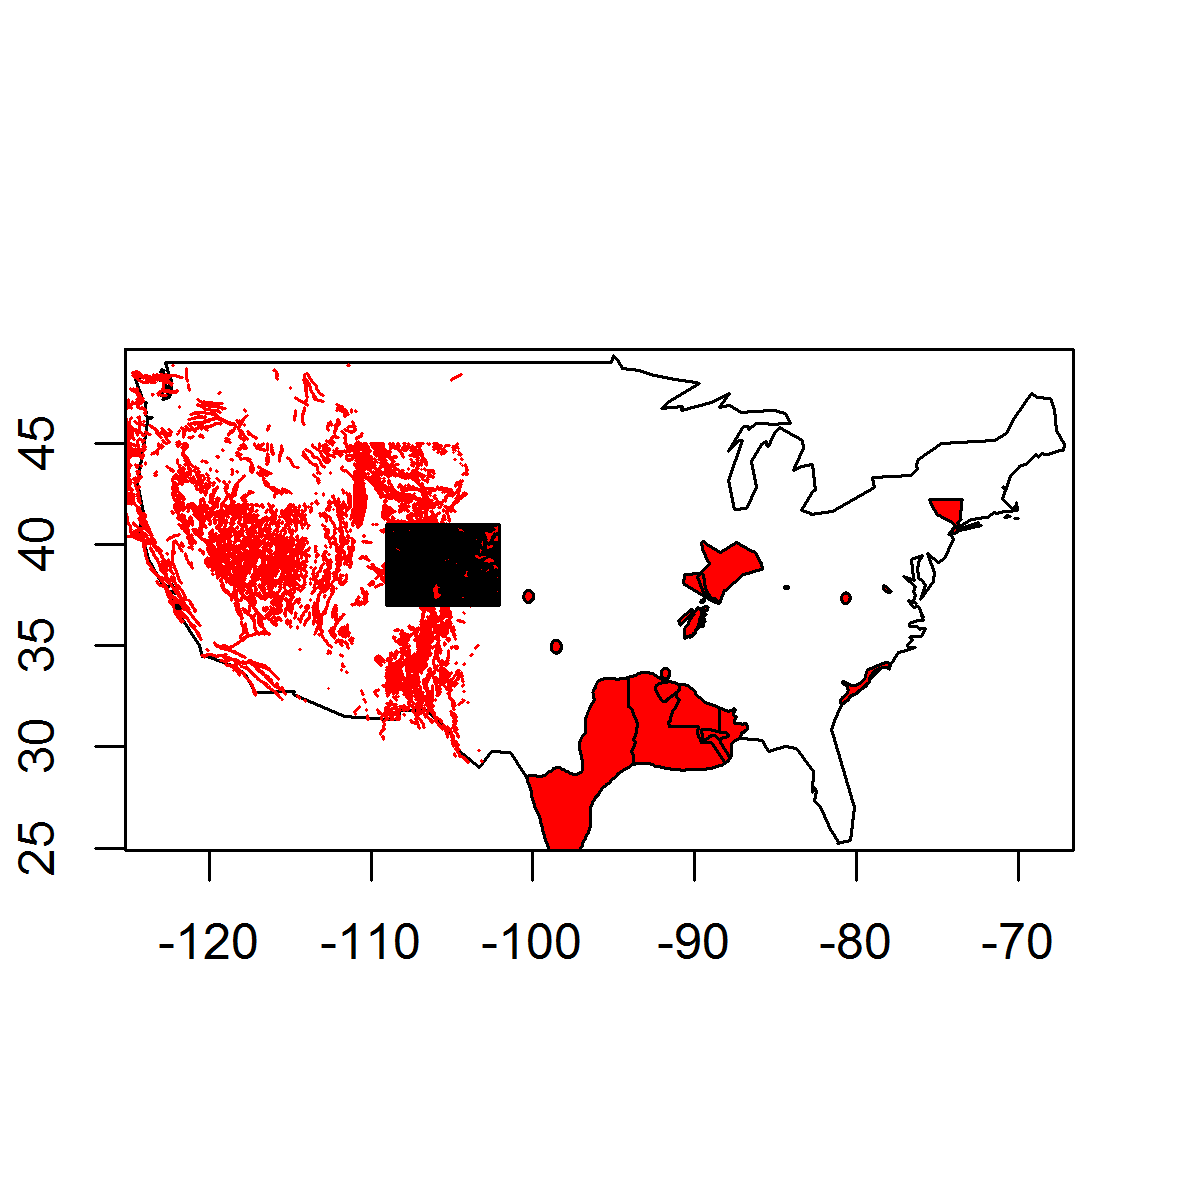
\includegraphics{faultlinefig}
   \caption{An example of querying and discovering multiple
   spatial datasets on ScienceBase. In this case, faultlines 
   across the U.S. The variability in data formats (some lines, some polygons)
   is intentionally included to show both data variability, and quick discovery 
   of different data types across various regions.}
   \label{figure:faultlinefig}
 \end{figure}

\subsection{ScienceBase authentication}

In addition to the large collection of open, reusable datasets and
useful metadata ScienceBase has to offer, it is
also a platform for sharing and collaboration on private, in-progress
data available only through authenticated access. To enable
private data contribution and access,
\pkg{sbtools} has built-in support for persistent
authentication of R sessions.

In \pkg{sbtools}, users can log into ScienceBase with their ScienceBase username
and password using the function \code{authenticate\_sb()}. To prevent plain-text
passwords from being saved in the R command history, the password can be typed
into a pop-up window. \pkg{sbtools} only stores the authenticated session,
thereby maintaining the confidentiality of the user's credentials. ScienceBase
sessions remain active for roughly one hour and are renewed each time a request
is made. \pkg{sbtools} makes a best effort to supply the user with meaningful
error messages when a session may have expired.

\noindent\rule{\textwidth}{0.4pt}
%Authentication in sbtools
\begin{example}
#to start an authenticated session
> authenticate_sb('username@usgs.gov') #password entered into pop-up window
> is_logged_in()
[1] TRUE
> session_logout()
> is_logged_in()
[1] FALSE
\end{example}
\noindent\rule{\textwidth}{0.4pt}

Most functions in \pkg{sbtools} can be used both anonymously and when
authenticated. This includes all data retrieval and query functions. The
behavior of these functions depends on the user's authentication status and
access permissions. For example, when trying to access a private item using
\code{item\_get()}, you must be authenticated or will receive an error that the
item is missing. To maintain privacy, ScienceBase does not differentiate between
a missing item and an item you don't have permission to access. Search is also
dependent on authentication status. When querying items with \code{query\_sb()},
public items are always visible while private items are invisible unless
authenticated.

\noindent\rule{\textwidth}{0.4pt}
\begin{example}
#Attempt to get a private item without authentication
> item_get('55de0027e4b0518e354dfcf0')
 Error: Item not found for ID=55de0027e4b0518e354dfcf0. Either the
 item does not exist or the item is secured and requires authentication to access.

#Get private item while authenticated
> authenticate_sb('username@usgs.gov')
> item_get('55de0027e4b0518e354dfcf0')
 <ScienceBase Item>
  Title: Example Private Item
  Creator/LastUpdatedBy:     username@usgs.gov / username@usgs.gov
  Provenance (Created / Updated):  2015-08-26T18:06:31Z / 2015-12-30T14:59:27Z
  Children: FALSE
  Item ID: 55de0027e4b0518e354dfcf0
  Parent ID: 54257d8fe4b0e641df8b50af

#Search results include user's private items when authenticated
> query_sb(list(q = 'username@usgs.gov'))
 <ScienceBase Item>
  Title: Example Private Item
  Creator/LastUpdatedBy:     username@usgs.gov / username@usgs.gov
  Provenance (Created / Updated):  2015-08-26T18:06:31Z / 2015-12-30T14:59:27Z
  Children: FALSE
  Item ID: 55de0027e4b0518e354dfcf0
  Parent ID: 54257d8fe4b0e641df8b50af

#Search results hide private items when not authenticated
> session_logout()
> query_sb(list(q = 'username@usgs.gov'))
list()
\end{example}
\noindent\rule{\textwidth}{0.4pt}

The authentication status can be quickly checked and updated 
with a few helper functions.

\noindent\rule{\textwidth}{0.4pt}
\begin{example}
#See if user is authenticated to SB
> is_logged_in()
[1] TRUE

#Get details of authenticated session 
> session_details()
$fullDisplayName
[1] "User McUseface [username@usgs.gov]"
$isLoggedIn
[1] TRUE
$displayName
[1] "User McUseface"
$email
[1] "username@usgs.gov"
$username
[1] "username@usgs.gov"

#Renew a session to prevent expiration after 1 hour
> session_renew()
\end{example}
\noindent\rule{\textwidth}{0.4pt}

\subsection{Data editing and upload API}
For authenticated users, \pkg{sbtools} can support
the full data lifecycle. This includes the creation, editing and removal
of items. Because item editing and creation cannot be done anonymously,
this functionality only works while authenticated.

To create new items, the only required input to \code{item\_create} is "title".
The "Parent Item" may also be specified. New items, by default, inhert the privacy 
settings of their parent item. All users have a personal home folder
(called "My Items" on the ScienceBase website) that serves as the default parent
item for new items. The unique identifier of a user`s home folder can be
retrieved with the function \code{user\_id()}.

\noindent\rule{\textwidth}{0.4pt}
\begin{example}
#create new item, by default under "My Items" parent
> new_item = item_create(title = 'new test item')
> new_item
<ScienceBase Item>
  Title: new test item
  Creator/LastUpdatedBy:     username@usgs.gov / username@usgs.gov
  Provenance (Created / Updated):  2016-01-27T19:48:28Z / 2016-01-27T19:48:28Z
  Children: FALSE
  Item ID: 56a91f0ce4b0b28f1184dda8
  Parent ID: 54257d8fe4b0e641df8b50af
\end{example}
\noindent\rule{\textwidth}{0.4pt}

Once an item is created, an authenticated user can edit the metadata or attach
data files to that item.

\noindent\rule{\textwidth}{0.4pt}
\begin{example}
#give the item a new title
> edited_item = item_update(new_item, list(title = 'new updated item'))
> edited_item
<ScienceBase Item>
  Title: new updated item
  Creator/LastUpdatedBy:     lwinslow@usgs.gov / lwinslow@usgs.gov
  Provenance (Created / Updated):  2016-01-27T19:48:28Z / 2016-01-27T19:50:21Z
  Children: FALSE
  Item ID: 56a91f0ce4b0b28f1184dda8
  Parent ID: 54257d8fe4b0e641df8b50af

#append files to the item
> item_list_files(new_item)
data frame with 0 columns and 0 rows

> item_append_files(edited_item, 'test.dat')
> item_list_files(edited_item)
      fname size     url
1 README.md 1282     https://www.sciencebase.gov/[long URL truncated]
\end{example}
\noindent\rule{\textwidth}{0.4pt}

Functions are also provided to modify and delete attached files and to delete
entire items.

\noindent\rule{\textwidth}{0.4pt}
\begin{example}
#list currently attached files
> item_list_files(edited_item)
      fname size     url
1 README.md 1282     https://www.sciencebase.gov/[long URL truncated]

#selectively replace files. all = FALSE replaces files one by one;
#otherwise all files are removed before uploading the new files
> item_replace_files(new_item, 'README.md', all = FALSE)
> item_list_files(edited_item)
      fname size     url
1 README.md 608     https://www.sciencebase.gov/[long URL truncated]

#delete item. use with caution; there is no confirmation check
> item_rm(edited_item)
> item_get(edited_item)
Error: Item not found for ID=56a91f0ce4b0b28f1184dda8. Either the item does
not exist or the item is secured and requires authentication to access.
\end{example}
\noindent\rule{\textwidth}{0.4pt}

\subsection{SB Item identifiers}
One advanced feature of ScienceBase is the ability to assign any
number of custom item identifiers to items. The custom identifiers are made up
of three parts: Scheme, Type and Key. Combined, these create a unique identifier.
There are some standard Schemes used in ScienceBase. For example, DOIs (Digital
Object Identifiers) are stored as item identifiers with the Scheme \\
"https://www.sciencebase.gov/vocab/category/item/identifier" and Type "DOI".

\pkg{sbtools} can edit and query custom item identifiers using
\code{item\_update\_identifier} and \code{query\_item\_identifier},
respectively.

\noindent\rule{\textwidth}{0.4pt}
\begin{example}
#create two items and assign custom identifiers
> ident_item = item_create(title = 'test data')
> item_update_identifier(ident_item, scheme = 'proj2', type = 'data', key = 'dataset1')
> ident_item = item_create(title = 'test publication')
> item_update_identifier(ident_item, scheme = 'proj2', type = 'publication', key = 'pdf1')

#query for created item
> query_item_identifier(scheme = 'proj2', type = 'publication', key = 'pdf1')
             title                       id
1 test publication 56a9371ee4b012c193aa3d65
\end{example}
\noindent\rule{\textwidth}{0.4pt}

The three-part identifier can be especially useful as a way to
organize and access project data. For example, all items within the same project
could be created with the same scheme and differing types or keys, allowing
users to query items within the project using custom tags that are meaningful to
that project.

\noindent\rule{\textwidth}{0.4pt}
\begin{example}
#query all items in 'proj2'
> query_item_identifier(scheme = 'proj2')
             title                       id
1 test publication 56a9371ee4b012c193aa3d65
2        test data 56a93777e4b012c193aa3d68

#query just data items for a project
> query_item_identifier(scheme = 'proj2', type = 'data')
      title                       id
1 test data 56a93777e4b012c193aa3d68
\end{example}
\noindent\rule{\textwidth}{0.4pt}
